\documentclass[submit]{harvardml}

\course{CS181-S23}
\assignment{Assignment \#5}
\duedate{11:59PM EST, April 27 2023}
\newcommand{\attr}[1]{\textsf{#1}}
\usepackage[OT1]{fontenc}
\usepackage{float}
\usepackage[colorlinks,citecolor=blue,urlcolor=blue]{hyperref}
\usepackage[pdftex]{graphicx}
\usepackage{subfig}
\usepackage{fullpage}
\usepackage{amsmath}
\usepackage{amssymb}
\usepackage{color}
\usepackage{todonotes}
\usepackage{listings}
\usepackage{common}
\usepackage{bm}
\usepackage{enumitem}
\usepackage{tikz}
\usepackage{xifthen}
\usepackage{soul}
\usepackage{framed}
\usetikzlibrary{automata,arrows,positioning,calc}

\usepackage[mmddyyyy,hhmmss]{datetime}

\definecolor{verbgray}{gray}{0.9}

\lstnewenvironment{csv}{
  \lstset{backgroundcolor=\color{verbgray},
  frame=single,
  framerule=0pt,
  basicstyle=\ttfamily,
  columns=fullflexible}}{}

\newcommand{\mueps}{\mu_{\epsilon}}
\newcommand{\sigeps}{\sigma_{\epsilon}}
\newcommand{\mugam}{\mu_{\gamma}}
\newcommand{\siggam}{\sigma_{\gamma}}
\newcommand{\muzp}{\mu_{p}}
\newcommand{\sigzp}{\sigma_{p}}
\newcommand{\gauss}[3]{\frac{1}{2\pi#3}e^{-\frac{(#1-#2)^2}{2#3}}}


\begin{document}
\begin{center}
{\Large Homework 5: Markov Decision Processes and Reinforcement Learning}\\
\end{center}

\subsection*{Introduction}

In this assignment, you will gain intuition for how MDPs and RL work.  For readings, we recommend Chapters 11 and 12 of the \href{https://github.com/harvard-ml-courses/cs181-textbook/blob/master/Textbook.pdf}{CS181 textbook} and the pre-lecture materials from April 11th and April 13th.

Please type your solutions after the corresponding problems using this
\LaTeX\ template, and start each problem on a new page.

Please submit the \textbf{writeup PDF to the Gradescope assignment `HW5'}. Remember to assign pages for each question.

Please submit your \textbf{\LaTeX\ file and code files to the Gradescope assignment `HW5 - Supplemental'}. 

You can use a \textbf{maximum of 2 late days} on this assignment.  Late days will be counted based on the latest of your submissions. 
\\

\begin{problem}[Markov Decision Processes, 20 pts]
In this problem, you will be working on building your conceptual understanding of MDPs.

\begin{enumerate}
    \item For the past few weeks in this course we have seen how \textit{latent variable models} can be fit using the EM algorithm. Recall that in the M-step, we maximize the ELBO with respect to the model parameters given our best guess for the probability distribution over the latent variables. One of the terms in the ELBO is the \textit{complete data likelihood}.
    \begin{enumerate}
        \item  The complete data likelihood for one latent variable model called pPCA is as follows:
    \begin{align*}
        p(Z_{1\cdots N}, Y_{1\cdots N}|\theta) = \prod_{n=1}^N p(Y_n, Z_n|\theta) = \prod_{n=1}^N p(Y_n|Z_n, \theta)p(Z_n)
    \end{align*}
    \textbf{Question:} Use what you know from the factorization of the complete data likelihood for pPCA to either draw, or describe in words, its associated graphical model.
    \item The complete data likelihood for a Hidden Markov Model (HMM) is as follows:
    \begin{align*}
        p(Z_{1\cdots N}, Y_{1\cdots N}|\theta, \mathcal{T}) &= \prod_{n=2}^N p(Y_1, Z_1|\theta)\prod_{n=1}^N p(Y_n, Z_n|Z_{n-1}; \theta, \mathcal{T})\\
        &= p(Y_1|Z_1; \theta)p(Z_1)\prod_{n=2}^N p(Y_n|Z_n;\theta)p(Z_n|Z_{n-1}, \mathcal{T})
    \end{align*}
    \textbf{Question:} How does the graphical model for the HMM differ from that for pPCA? Where do you see the Markov assumption coming into play?
    \end{enumerate}

    % \item In the following example, we translate a medical study of personal fitness into an MDP. We observe the participants’ performance on a number of physical activities and divide them into two categories: fit and unfit. Over 11 weeks, we observe how the number of fit and unfit participants change from week to week. In particular, we find that from week $n$ to week $n + 1$, 80\% of participants who started the week as unfit, stayed unfit and 60\% of participants who started the week as fit, became unfit. We formalize our observation in the following MDP.

    % \textbf{INSERT IMAGE}

    % \textbf{Question:} What design choices did we make in constructing our model? What are the pro’s and con’s of these choices? If we want to make different design choices, what additional data do we need to collect (e.g. what if we wanted a state space that had three different fitness levels)?

    \item In the following example, we translate a medical study of personal fitness into an MDP. We observe the participants' performance on a number of physical activities and divide them into two categories: \textit{fit} and \textit{unfit}. Every week we also ask participants whether they worked out or not. We define our MDP as follows:
    \begin{align*}
        \mathcal{S} &= \{\text{unfit}, \text{fit}\}\\
        \mathcal{A} &= \{\text{workout (Y), not workout (N)}\}\\
    \end{align*}
    
    \begin{center}
    \begin{tabular}{ |c|c|c|c| } 
         \hline
        $s_{n}$ & $a_{n}$ & $s_{n + 1}$ & $\mathcal{R}(s_n, a_n, s_{n + 1})$\\
         \hline
        \text{fit} & Y & \text{fit} & 0\\
        \text{fit} & Y & \text{unfit} & -2\\
        \text{fit} & N & \text{fit} & 2\\
        \text{fit} & N & \text{unfit} & -1\\
        \text{unfit} & Y & \text{fit} & 1\\
        \text{unfit} & Y & \text{unfit} & -1\\
        \text{unfit} & N & \text{fit} & 10\\
        \text{unfit} & N & \text{unfit} & -1\\
        \hline
    \end{tabular}
        \end{center}


\begin{center}
	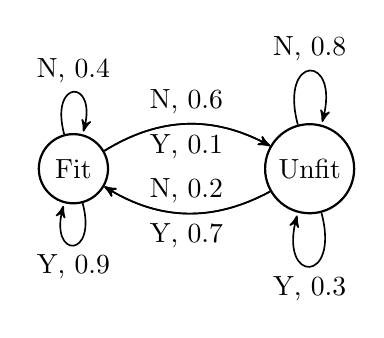
\begin{tikzpicture}[->, >=stealth', auto, semithick, node distance=3cm]
	\tikzstyle{every state}=[fill=white,draw=black,thick,text=black,scale=1]
	\node[state]    (A)                     {Fit};
	\node[state]    (B)[right of=A]   {Unfit};
	\path
	(A) edge[loop above]			node{N, $0.4$}	(A)
    (A) edge[loop below]            node{Y, $0.9$}  (A)
	(B) edge[loop above]			node{N, $0.8$}	(B)
    (B) edge[loop below]            node{Y, $0.3$}  (B)
    (A) edge[bend left,above]       node{N, $0.6$}  (B)
    (A) edge[bend left,below]       node{Y, $0.1$}  (B)
    (B) edge[bend left,above]       node{N, $0.2$}  (A)
    (B) edge[bend left,below]       node{Y, $0.7$}  (A);
	\end{tikzpicture}
\end{center}
    
    % \item Translate the MDP formalism above into statements about our grid world. What design choices did we make in defining this model? What are the pro’s and con’s of these choices? If we wanted to make different choices, what additional data do we need to collect, and how would these design choices affect the rest of the model? If we wanted to formalize our grid world as an MDP using $R:S \times A \rightarrow R$ how would we need to change our MDP definition?

    (continued on next page...)
\end{enumerate}
\end{problem}
\begin{framed}
    \noindent\textbf{Problem 1} (cont.)
   \begin{enumerate} 
       \setcounter{enumi}{1}
 \item \textbf{Question:} 
    \begin{enumerate}
        \item What is one design choice we made in this model? What is one pro and one con of this design choice?
        \item Suggest one modification we could make to this model and describe what additional data (if any) we would need to collect to make this modification. How would this modification affect the rest of the model?
        % \item How could we rewrite our reward function in the form $\mathcal{R}: \mathcal{S} \times \mathcal{A} \rightarrow \mathcal{R}$? What information would we lose in the process?
    \end{enumerate}
     \item Recall that \textit{planning} in an MDP is the process of finding a policy $\pi: \mathcal{S} \rightarrow \mathcal{A}$ that maximizes the agent's expected reward.
     
     \textbf{Question:}
     \begin{enumerate}
         \item In the MDP setting, why can't $\pi(s_{n})$ depend on the \textit{history} -- the values of previous states $s_{n - 1}, s_{n - 2}, ...$?
         % \item What is one real-life scenario where the independence of $\pi$ and the history is reasonable? How about a scenario where it is unreasonable?
         \item Is this assumption reasonable for our personal fitness MDP?
     \end{enumerate}
      
     
    \item Recall that the \textit{return} for a trajectory (a sequence of states and actions) of length $N$ is given by:
    \begin{align*}
        G = \sum_{n=1}^N \gamma^n R_n
    \end{align*}
    where $R_n$ is the reward collected at time $n$.

    \textbf{Question:} Why do we discount? Often we argue that discounting is needed if we allow infinite trajectories. Show that if $\gamma = 1$ and the trajectory is infinite then $G$ can be undefined.

    \item Recall that the value function of an MDP for state $s$ under policy $\pi$ is defined as follows:
    \begin{align*}
        V^\pi(s) = \mathbb{E}_{\pi}[G|Z_0 = s]
    \end{align*}
    where the expectation above is taken over all randomly varying quantities in $G$.

    \textbf{Question:}
    \begin{enumerate}
        \item In our personal fitness MDP what quantities that $G$ depends on are randomly varying?\\
        \textit{Hint:} Think about sources of randomness in your reward, transition and policy.
        \item Suppose the agent's policy $\pi$ is to exercise if in the \texttt{unfit} state and not exercise if in the \texttt{fit} state. Calculate $V^{\pi}(\text{fit})$ and $V^{\pi}(\text{unfit})$.
    \end{enumerate}
    

    \item Recall that the Q-function $Q^{\pi}: \mathcal{S} \times \mathcal{A} \rightarrow \mathcal{R}$ quantifies the value of a policy $\pi$ starting at state $s$, taking action $a$, and \textit{then} following policy $\pi$:
    \begin{align*}
        Q^{\pi}(s, a) = \mathbb{E}_\pi [G|Z_0 = s, A_0 = a]
    \end{align*}

    \textbf{Question:} Assuming that the agent follows the same policy as in the previous question, calculate $Q^{\pi}(\text{fit}, \text{Y})$, $Q^{\pi}(\text{fit}, \text{N})$, $Q^{\pi}(\text{unfit}, \text{Y})$, $Q^{\pi}(\text{unfit}, \text{N})$.
    \end{enumerate}
\end{framed}

\begin{problem}[Reinforcement Learning, 20 pts]
  In 2013, the mobile game \emph{Flappy Bird} took the world by storm. You'll be developing a Q-learning agent to play a similar game, \emph{Swingy Monkey} (See Figure~\ref{fig:swingy}).  In this game, you control a monkey that is trying to swing on vines and avoid tree trunks.  You can either make him jump to a new vine, or have him swing down on the vine he's currently holding.  You get points for successfully passing tree trunks without hitting them, falling off the bottom of the screen, or jumping off the top.  There are some sources of randomness: the monkey's jumps are sometimes higher than others, the gaps in the trees vary vertically, the gravity varies from game to game, and the distances between the trees are different.  You can play the game directly by pushing a key on the keyboard to make the monkey jump.  However, your objective is to build an agent that \emph{learns} to play on its own. 
  
   You will need to install the \verb|pygame| module
  (\url{http://www.pygame.org/wiki/GettingStarted}).
  

\textbf{Task:}
Your task is to use Q-learning to find a policy for the monkey that can navigate the trees.  The implementation of the game itself is in file \verb|SwingyMonkey.py|, along with a few files in the \verb|res/| directory.  A file called \verb|stub.py| is the starter code for setting up your learner that interacts with the game.  This is the only file you need to modify (but to speed up testing, you can comment out the animation rendering code in \verb|SwingyMonkey.py|). You can watch a YouTube video of the staff Q-Learner playing the game at \url{http://youtu.be/l4QjPr1uCac}.  It figures out a reasonable policy in a few dozen iterations.
You'll be responsible for implementing the Python function  \verb|action_callback|. The action callback will take in a dictionary that describes the current state of the game and return an action for the next time step.  This will be a binary action, where 0 means to swing downward and 1 means to jump up.  The dictionary you get for the state looks like this:
\begin{csv}
{ 'score': <current score>,
  'tree': { 'dist': <pixels to next tree trunk>,
            'top':  <height of top of tree trunk gap>,
            'bot':  <height of bottom of tree trunk gap> },
  'monkey': { 'vel': <current monkey y-axis speed>,
              'top': <height of top of monkey>,
              'bot': <height of bottom of monkey> }}
\end{csv}
All of the units here (except score) will be in screen pixels. Figure~\ref{fig:swingy-ann} shows these graphically. 
Note that since the state space is very large (effectively continuous), the monkey's relative position needs to be discretized into bins. The pre-defined function \verb|discretize_state| does this for you.

\textbf{Requirements}
\\
\textit{Code}: First, you should implement Q-learning with an
$\epsilon$-greedy policy yourself. You can increase the performance by
trying out different parameters for the learning rate $\alpha$,
discount rate $\gamma$, and exploration rate $\epsilon$. \emph{Do not use outside RL code for this assignment.} Second, you should use a method of your choice to further improve the performance. This could be inferring gravity at each epoch (the gravity varies from game to game), updating the reward function, trying decaying epsilon greedy functions, changing the features in the state space, and more. One of our staff solutions got scores over 800 before the 100th epoch, but you are only expected to reach scores over 50 before the 100th epoch. {\bf Make sure to turn in your code!} \\\\
\textit{Evaluation}: In 1-2 paragraphs, explain how your agent performed and what decisions you made and why. Make sure to provide evidence where necessary to explain your decisions. You must include in your write up at least one plot or table that details the performances of parameters tried (i.e. plots of score vs. epoch number for different parameters).
\\\\
\textit{Note}: Note that you can simply discretize the state and action spaces and run the Q-learning algorithm. There is no need to use complex models such as neural networks to solve this problem, but you may do so as a fun exercise.

\end{problem}
\begin{figure}[H]
    \centering%
    \subfloat[SwingyMonkey Screenshot]{%
        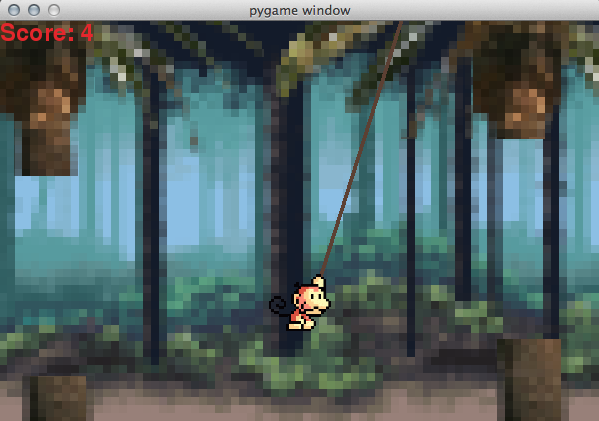
\includegraphics[width=0.48\textwidth]{figures/swingy}
        \label{fig:swingy}
    }\hfill
    \subfloat[SwingyMonkey State]{%
        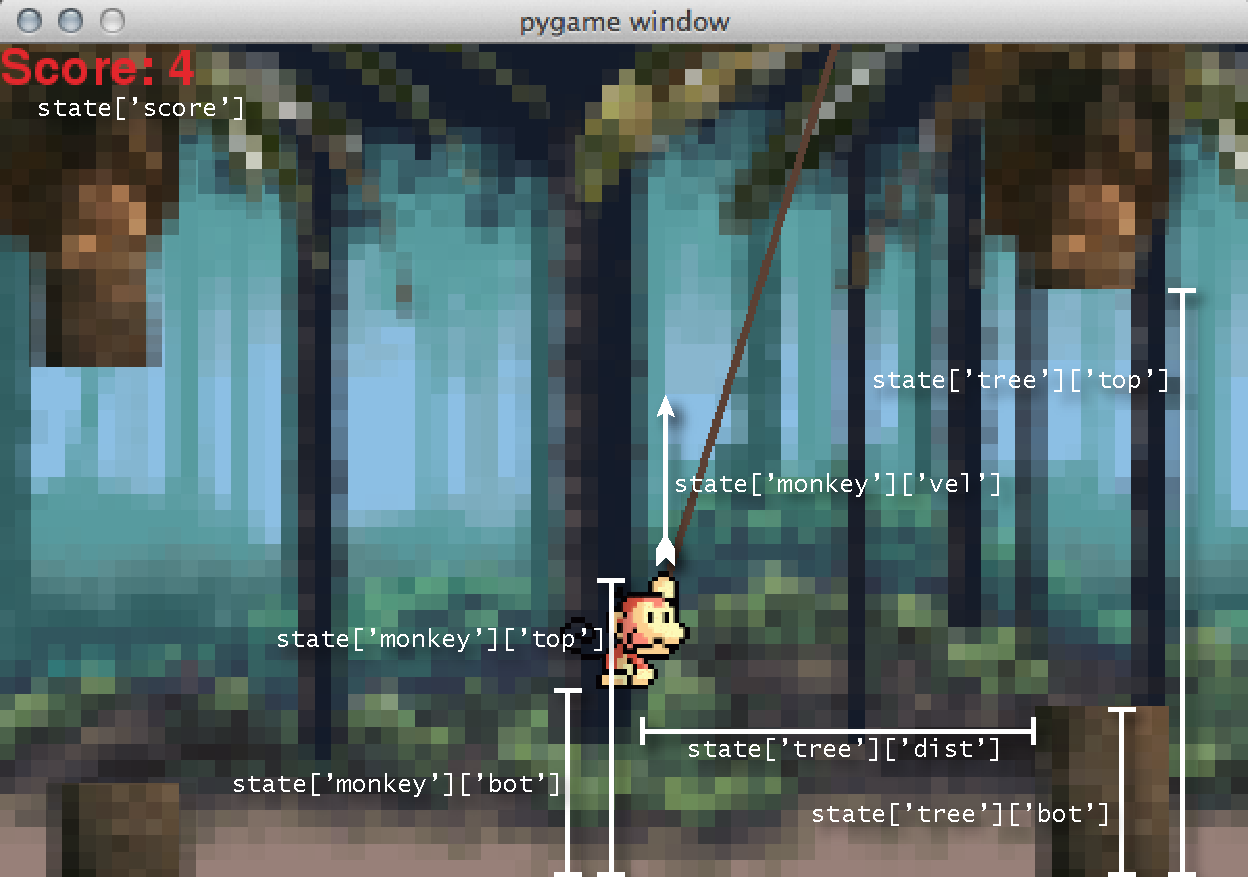
\includegraphics[width=0.48\textwidth]{figures/swingy-ann}
        \label{fig:swingy-ann}
    }
    \caption{(a) Screenshot of the Swingy Monkey game.  (b) Interpretations of various pieces of the state dictionary.}
\end{figure}
\newpage
\begin{problem}[Impact Question: Assessing the energy consumption of data centers and understanding a RL approach to optimize it, 3.5 pts]
Every computation consumes energy. Over the past decades large scale data centers have been built which are significant energy consumers. Consequently, every computation is costly.  

\begin{enumerate}
    \item \textbf{Energy consumption}: How much energy do data centers consume globally per year? And what's their share in global energy consumption? (1 point)
    \item \textbf{Consumption optimization with RL}: How would you formulate a RL model which enables the optimization of the load of a data center? Describe the main elements of your model (state space, action space, reward). (1.5 points)\\
   \textit{Hint:} This \href{https://people.csail.mit.edu/alizadeh/papers/deeprm-hotnets16.pdf}{RL Paper} provides background information for this.
   \item \textbf{Alternatives}: List one alternative idea on how to reduce the climate impact of data centers. (1 point)
\end{enumerate}
\end{problem}
    
%%%%%%%%%%%%%%%%%%%%%%%%%%%%%%%%%%%%%%%%%%%%%
% Name and Calibration
%%%%%%%%%%%%%%%%%%%%%%%%%%%%%%%%%%%%%%%%%%%%%
\newpage
\subsection*{Name}
\subsection*{Collaborators and Resources}
Whom did you work with, and did you use any resources beyond cs181-textbook and your notes?
\subsection*{Calibration}
Approximately how long did this homework take you to complete (in hours)? 
\end{document}
